\documentclass[../sparc.tex]{subfiles}
\graphicspath{{\subfix{../images/}}}
\begin{document}

%%%%%%%%%%%%%%%%%%%%%%%%%%%%%%%%%%%%%%%%%%%%%%%%%%%%%%%%%%%%%%%%%%%%%%%%%%%%%%%%
\section{Шина I2C}
\label{section:i2c}
\index{Электроника!Шина I2C}
\newglossaryentry{I2C}{name=I2C, description={Inter-Integrated Circuit}}

\newglossaryentry{USB}{name=USB, description={Universal Serial Bus --
    ``Универсальная последовательная шина.''}}

\newglossaryentry{PCI}{name=PCI, description={Peripheral component interconnect
    -- ``взаимосвязь периферийных компонентов''}}

\newglossaryentry{I/O}{name=I/O, description={I/O -- ``Input/Output''}}

\textit{\gls{I2C}} также иногда называемя $I^{2}C$ (читается ``ай-квадрат-си''),
-- шина передачи данных, используемая для связи между интегральными схемами
внутри электронных приборов. Давайте рассмотрим во-первых, что такое ``шина
передачи данных''. Если кратко, то \textit{шина} (англ. \textit{bus}) в
архитектуре компьютера -- это некое соединение, служащее для передачи данных
между функциональными блоками коммьютера.

Шины передачи данных условно можно разделить на две крупные категории --
\textit{внешние} шины и \textit{внутренние} шины.

К внешним шинам можно отнести наверняка знакомый многим из вас \gls{USB} --
данная шина используется для соединения внешних устройств (таких, как Arduino,
клавиатура, мышь, принтер и т.п.) с компьютером.  Подобные шины как правило
имеют стандартизированный разъём и достаточно большую длину провода.

К внутренним шинам относится уже упомянутый выше \gls{I2C} и \gls{PCI}/PCI
Express (используемой например для подключения сетевой карты к материнской плате
компьютера.)  Внутренние шины обычно подразумевают передачу данных на короткие
дистации, оперативное отключение/подключение компонентов не предусмотрено и,
следовательно, некоторые из внутренних шин не имеют своего специализированного
разъёма и бывают просто распаены прямо на плате.

Максимальная длина соединения между компонентами на шине \gls{I2C} не должна
превышать 30 сантиметров, в противном случае данные будут передаваться
ненадёжно.

\gls{I2C} имеет достаточно низкую скорость передачи данных (не более 5МБит/с)
между устройствами. У каждого устройства есть свой \textit{адрес} на шине --
можно сказать, его поядковый номер. На одну шину можно подключить до 127
устройств с уникальными адресами. При этом, на шине одно устройство является
ведущим (как правило, это какой-либо микроконтроллер) и остальные устройства
являются ведомыми.

На рис. \ref{fig:i2c-schematics} показана схема шины \gls{I2C}. Как можно видеть
на рисунке, шина использует всего две линии для передачи данных -- ``Serial Data
Line'' (\textbf{SDL}) и ``Serial Clock Line'' (\textbf{SCL}). Обе линии
подтянуты через резисторы \textbf{$R_p$} к напряжению питания (\textbf{Vdd}). На
схеме ``$\mu$C\\Controller'' -- это ведущее устройство, остальные же, указанные как
``Target'', являются ведомыми.

\begin{figure}[H]
  \centering
  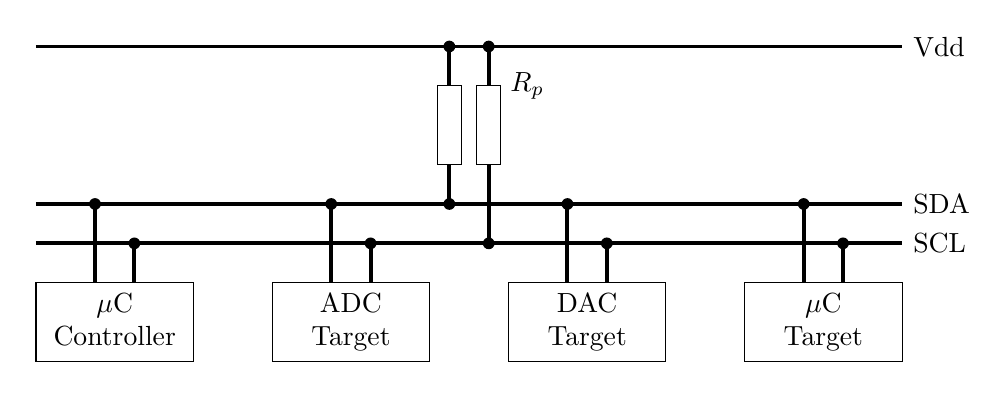
\begin{tikzpicture}
    \draw[draw=black] (0, 2) rectangle ++(2, 1) node[pos=.5] {%
      \begin{tabular}{c}%
        $\mu$C\\Controller%
    \end{tabular}};
    \draw[draw=black] (3, 2) rectangle ++(2, 1) node[pos=.5] {
      \begin{tabular}{c}
        ADC\\Target
    \end{tabular}};
    \draw[draw=black] (6, 2) rectangle ++(2, 1) node[pos=.5] {
      \begin{tabular}{c}
        DAC\\Target
    \end{tabular}};
    \draw[draw=black] (9, 2) rectangle ++(2, 1) node[pos=.5] {
      \begin{tabular}{c}
        $\mu$C\\Target
    \end{tabular}};

    %% Horizontal lines.
    \draw [line width=0.5mm] (0, 3.5) -- (11, 3.5) node[right] {SCL};
    \draw [line width=0.5mm] (0, 4.0) -- (11, 4.0) node[right] {SDA};
    \draw [line width=0.5mm] (0, 6.0) -- (11, 6.0) node[right] {Vdd};

    %% Vertical lines.
    \foreach \a/\b in {0.75/1.25, 3.75/4.25, 6.75/7.25, 9.75/10.25} {
      \draw [line width=0.5mm] (\a, 3) -- (\a, 4) node[circle,fill,inner sep=1.5pt]{};
      \draw [line width=0.5mm] (\b, 3) -- (\b, 3.5) node[circle,fill,inner sep=1.5pt]{};
    };

    \draw[line width=0.5mm] (5.25, 4) node[circle,fill,inner sep=1.5pt]{}
    -- (5.25, 6) node[circle,fill,inner sep=1.5pt]{};
    \draw[line width=0.5mm] (5.75, 3.5) node[circle,fill,inner sep=1.5pt]{}
    -- (5.75, 6) node[circle,fill,inner sep=1.5pt]{};

    \draw[draw=black, fill=white] (5.1, 4.5) rectangle ++(0.3, 1);
    \draw[draw=black, fill=white] (5.6, 4.5) rectangle ++(0.3, 1) node[right] {$R_p$};

  \end{tikzpicture}
  \caption{Устройство шины \gls{I2C}.}
  \label{fig:i2c-schematics}
\end{figure}

Стандартной библиотекой для работы с протоколом I2C является
\href{https://www.arduino.cc/reference/en/language/functions/communication/wire/}{Wire}.
Библиотека позволяет работать с I2C-устройствами.

\begin{table}[h]
  \centering
  \begin{tabular}{ | c | c | c | }
    \hline
    \multirow{2}{8em}{\textbf{Плата}} & \multicolumn{2}{c|}{\textbf{Порты I2C}} \\
    \cline{2-3}
    & \textbf{SDA} & \textbf{SCL} \\
    \hline
    Nano & A4 & A5 \\
    \hline
    UNO R3 & A4 & A5 \\
    \hline
    Leonardo & D2 & D3 \\
    \hline
    Mega 2560 Rev3 & D20 & D21 \\
    \hline
    Due & D20 & D21 \\
    \hline
  \end{tabular}
  \caption{I2C-порты на разных платформах Arduino.}
  \label{table:i2c-pins}
\end{table}

Из-за аппаратных различий между платформами Arduino, I2C-порты на разных видах
Arduino могут отличаться. Например, таблица \ref{table:i2c-pins} приводит
несколько примеров.

%%%%%%%%%%%%%%%%%%%%%%%%%%%%%%%%%%%%%%%%%%%%%%%%%%%%%%%%%%%%%%%%%%%%%%%%%%%%%%%%
\subsection{I2C-сканер}
\label{section:i2c-scanner}
\index{Электроника!Шина I2C!I2C-сканер}

Для того, чтобы быстро найти подключенные к шине \gls{I2C} устройства,
существует такой класс программ, как ``I2C-сканеры''.  Пример такой программы
можно найти на официальном сайте
Arduino. \footnote{\url{https://playground.arduino.cc/Main/I2cScanner/}}

Также более ``продвинутый'' I2C-сканер можно установить из менеджера библиотек
Arduino IDE -- он доступен по названию ``I2C\_Scanner''.

Подобные сканеры обычно выводят на компьютер через \texttt{Serial} список (или
таблицу) адресов I2C-устройств, подключенных к микроконтроллеру.

%%%%%%%%%%%%%%%%%%%%%%%%%%%%%%%%%%%%%%%%%%%%%%%%%%%%%%%%%%%%%%%%%%%%%%%%%%%%%%%%
\subsection{Пример I2C устройства: PCF8574}
\index{Электроника!Шина I2C!PCF8574}

\begin{figure}[H]
  \centering
  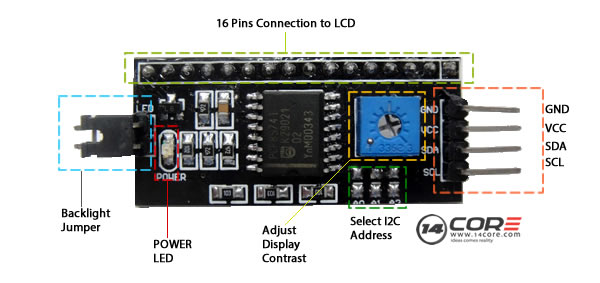
\includegraphics[width=12cm]{I2C-PCF8574-LCD-ADAPTER}
  \caption{I2C-адаптер ЖК-дисплея LCM1602-I2C на базе расширителя портов
    PCF8574.}
  \label{fig:i2c-pcf8574-lcd-adapter}
\end{figure}

Существует масса примеров устройств, которые могут подключаться к
микроконтроллеру по шине \gls{I2C}.  Одним из таких устройств является
расширитель портов ввода-вывода PCF8574.  Это специальная микросхема, которая
позволяет по шине I2C выставлять и считывать цифровое значение на каждой из 8
выходных ножек, таким образом потенциально управляя восемью устройствами.  Иными
словами, PCF8574 является восмиканальным расширителем портов ввода/вывода.

На базе PCF8574 построен специальный адаптер для подключения
жидкокристаллического (ЖК) текстового дисплея
(см. рис. \ref{fig:i2c-pcf8574-lcd-adapter}), позволяющий управлять дисплеем
через шину I2C.  Большинство ЖК-дисплеев имеют уже припаянный к нему I2C-модуль,
либо же подобный модуль можно купить и припаять отдельно.  Некоторые модели
дисплеев изначально имеют I2C-интерфейс и отдельного модуля для них не
требуется, так как необходимая ``обвязка'' уже распаяна прямо на плате дисплея.

В данном разделе, чтобы разобраться с шиной I2C, мы с вами попробуем
использовать расширитель портов, как на рис. \ref{fig:i2c-pcf8574-lcd-adapter},
для управления светодиодами.  Существуют уже готовая Arduino-библиотека для
работы
PCF8574\footnote{\url{https://www.arduino.cc/reference/en/libraries/pcf8574/}},
однако мы будем использовать только встроенную в Arduino IDE библиотеку
``Wire''\footnote{\url{https://www.arduino.cc/reference/en/language/functions/communication/wire/}}.

Обратите внимание, что модуль на рис. \ref{fig:i2c-pcf8574-lcd-adapter} имеет
область с тремя группами контактов (``A0'', ``A1'' и ``A2''), помеченную на
рисунке, как ``Select I2C Address'' -- через замыкание контактов путём впаивания
перемычек можно менять адрес данного I2C-устройства.  Имея три места под
перемычки, мы получаем $2^3 = 8$ возможных комбинаций перемычек.

\begin{table}[H]
  \centering
  \begin{tabular}{
      %% A2-A0
      | c | c | c
      %% A6-A0
      | c | c | c | c | c | c | c
      %% R/W
      | c
      %% Address
      | c
      | }
    \hline
    \multicolumn{3}{|c|}{\textbf{Подключение пинов}}
    & \multicolumn{8}{|c|}{\textbf{Конфигурация адреса}}
    & \multirow{2}{2em}{\textbf{Адрес I2C}} \\
    \textbf{A2}
    & \textbf{A1}
    & \textbf{A0}
    & \textbf{A6}
    & \textbf{A5}
    & \textbf{A4}
    & \textbf{A3}
    & \textbf{A2}
    & \textbf{A1}
    & \textbf{A0}
    & \textbf{R/W}
    &   \\
    \hline
    $V_{SS}$ & $V_{SS}$ & $V_{SS}$ & 0 & 1 & 0 & 0 & 0 & 0 & 0 & -- & \texttt{0x20} \\
    \hline
    $V_{SS}$ & $V_{SS}$ & $V_{DD}$ & 0 & 1 & 0 & 0 & 0 & 0 & 1 & -- & \texttt{0x21} \\
    \hline
    $V_{SS}$ & $V_{DD}$ & $V_{SS}$ & 0 & 1 & 0 & 0 & 0 & 1 & 0 & -- & \texttt{0x22} \\
    \hline
    $V_{SS}$ & $V_{DD}$ & $V_{DD}$ & 0 & 1 & 0 & 0 & 0 & 1 & 1 & -- & \texttt{0x23} \\
    \hline
    $V_{DD}$ & $V_{SS}$ & $V_{SS}$ & 0 & 1 & 0 & 0 & 1 & 0 & 0 & -- & \texttt{0x24} \\
    \hline
    $V_{DD}$ & $V_{SS}$ & $V_{DD}$ & 0 & 1 & 0 & 0 & 1 & 0 & 1 & -- & \texttt{0x25} \\
    \hline
    $V_{DD}$ & $V_{DD}$ & $V_{SS}$ & 0 & 1 & 0 & 0 & 1 & 1 & 0 & -- & \texttt{0x26} \\
    \hline
    $V_{DD}$ & $V_{DD}$ & $V_{DD}$ & 0 & 1 & 0 & 0 & 1 & 1 & 1 & -- & \texttt{0x27} \\
    \hline
  \end{tabular}
  \caption{Адресация модуля LCM1602-I2C.}
  \label{table:i2c-lcm1602-addressing}
\end{table}

В таблице \ref{table:i2c-lcm1602-addressing} показаны возможные комбинации
перемычек и соответствующие адреса модуля.\footnote{Источник:
\url{https://static.chipdip.ru/lib/807/DOC015807788.pdf}}

Как мы говорили выше, на самом деле на шине I2C адрес устройства кодируется
восемью битами, где семь бит (\texttt{A6-A0}) являются собственно сами адресом
устройства, а самый младший бит (\texttt{R/W}) кодирует направление передачи --
от устройства, или на устройство.  Изменение значений на пинах A0-A2 (первые три
столбца таблицы \ref{table:i2c-lcm1602-addressing}) меняет I2C-адрес устройства:
$V_{DD}$ означает напряжение питания (``supply voltage''), $V_{SS}$ -- землю
(``supply ground'').  Биты A3-A6 имеют фиксированное значение.

\begin{figure}[H]
  \centering
  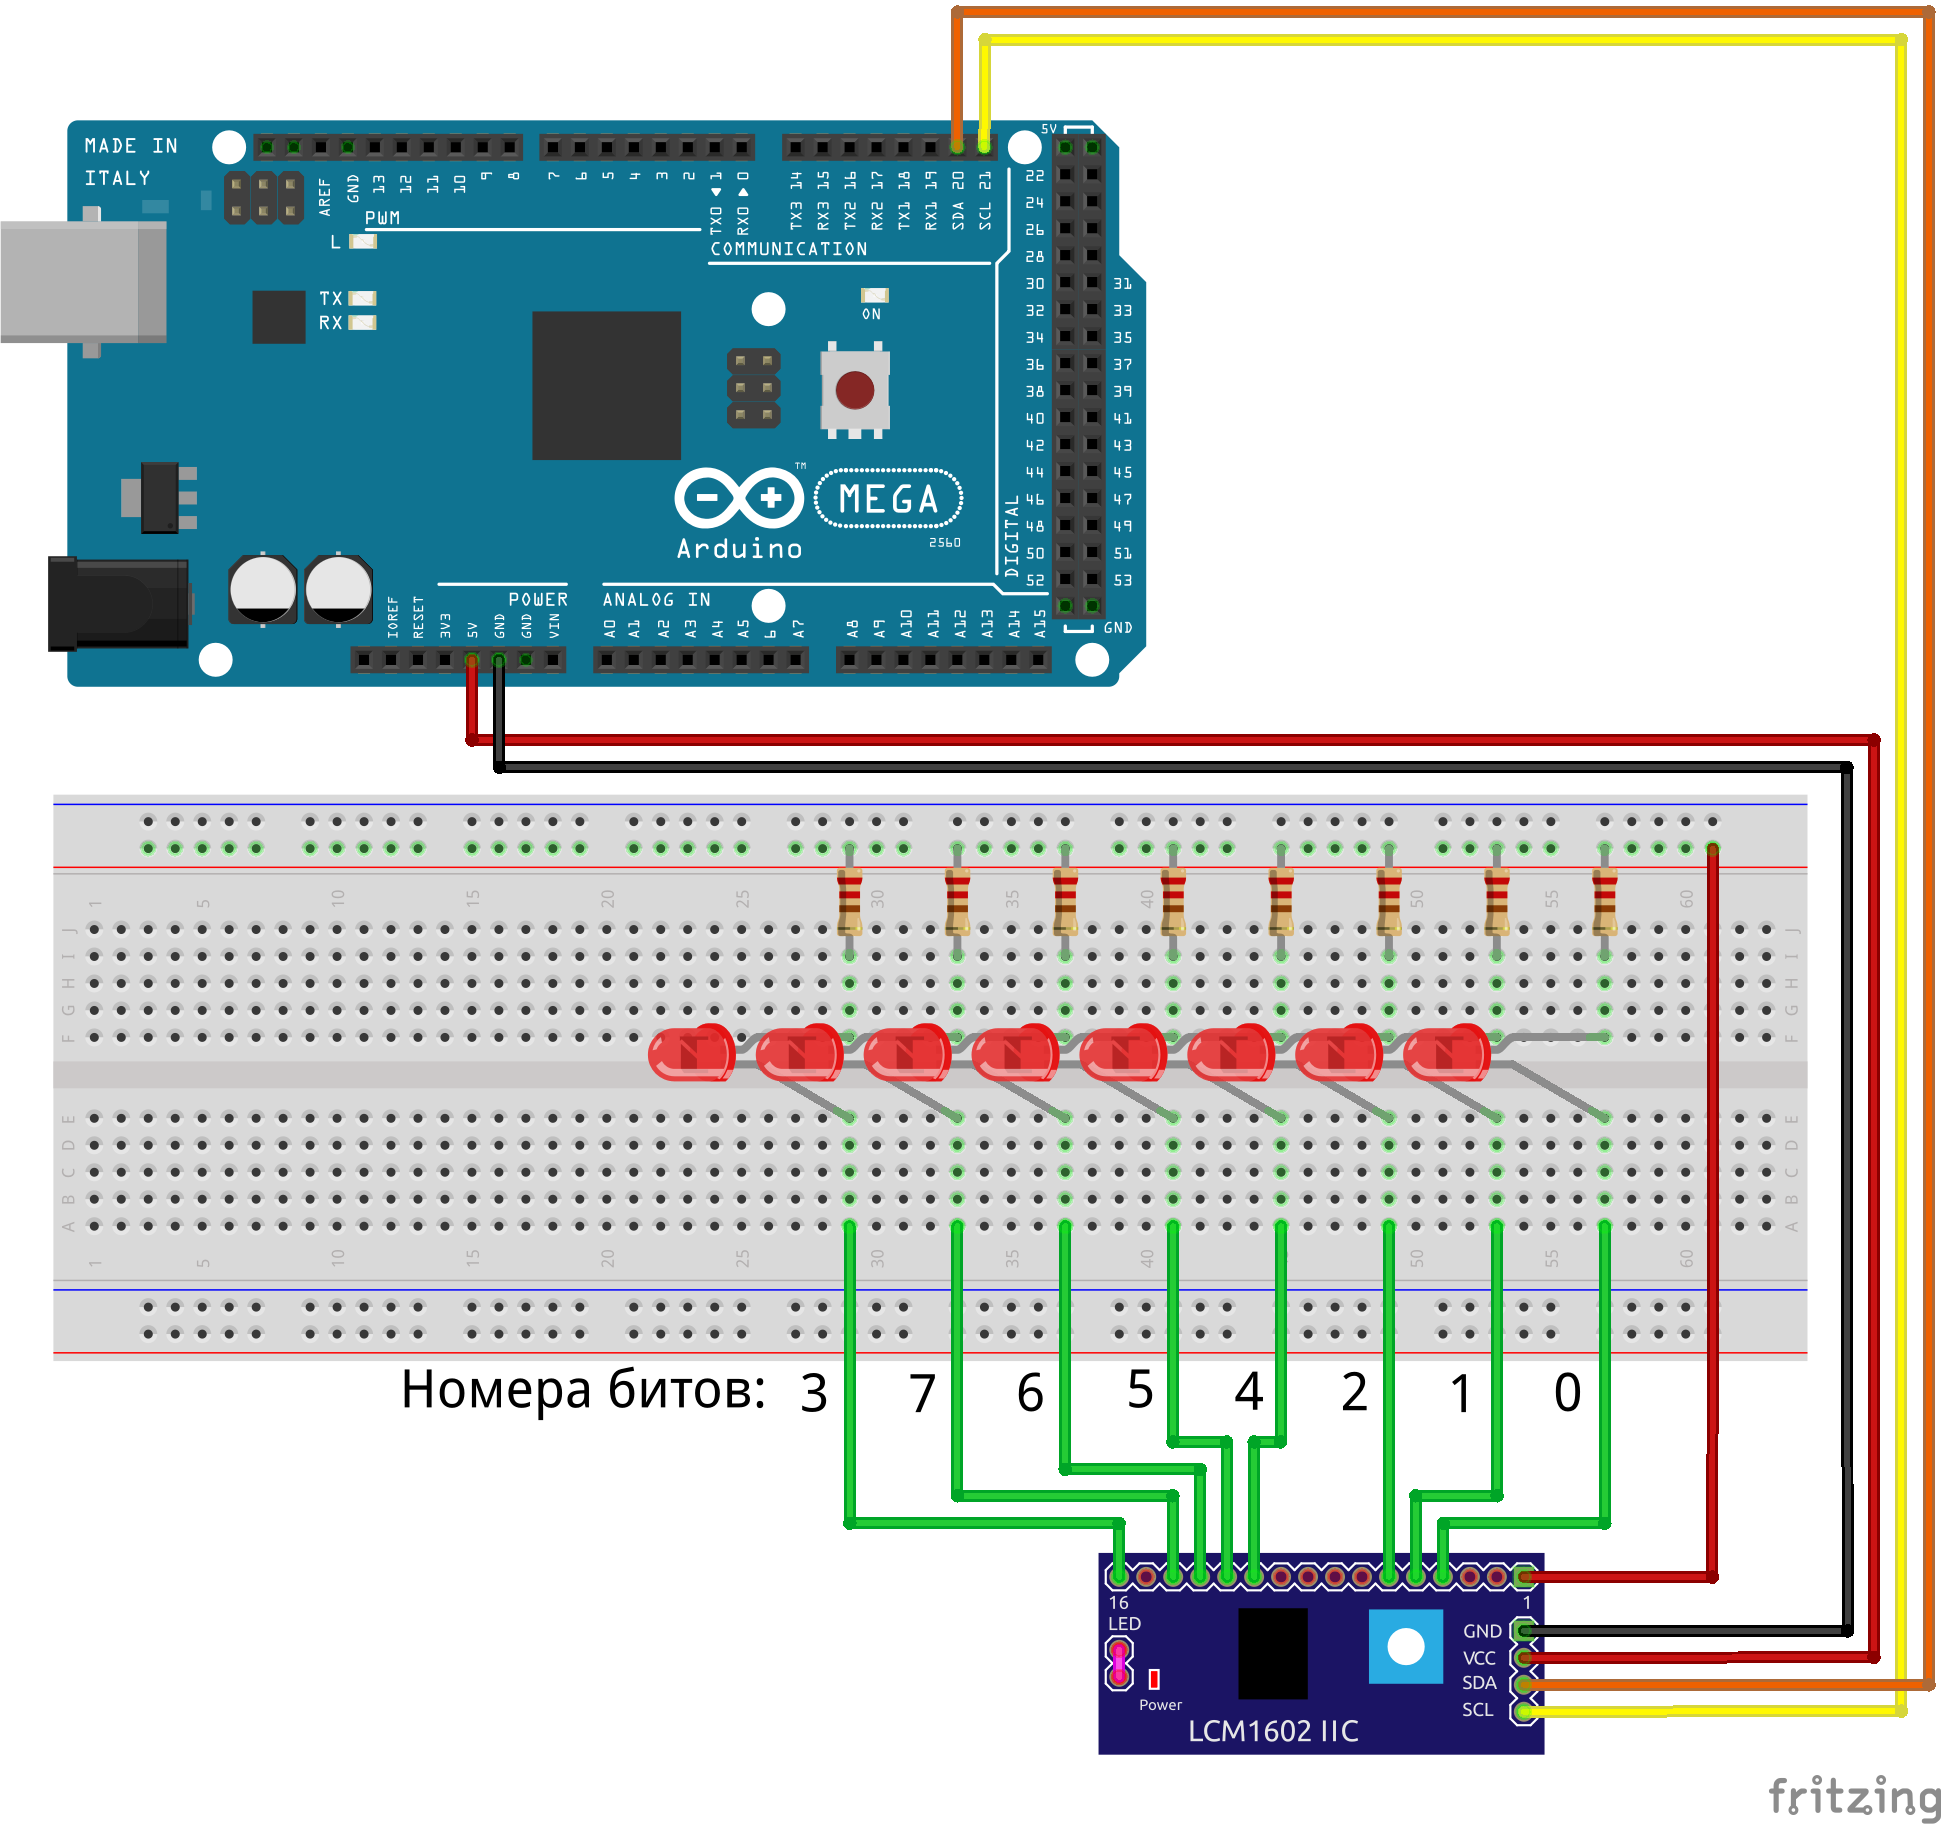
\includegraphics[width=12cm]{schematics/lcm1602-i2c-leds}
  \caption{I2C-модуль LCM1602 на базе микросхемы PCF8574 с подключенными восемью
    светодиодами.}
  \label{fig:lcm1602-i2c-leds}
\end{figure}

Для нашего проекта возьмём модуль, как на рис.
\ref{fig:i2c-pcf8574-lcd-adapter}, и подключим к каждой из восьми ножек
ввода/вывода один светодиод.  Биты, записываемые в модуль, будут напрямую
управлять состоянием светодиодов.  На рис. \ref{fig:lcm1602-i2c-leds} показан
один из возможных вариантов подключения компонентов для проекта.  Все резисторы
имеют номинал 220Ом.

Обратите внимание, что аноды светодиодов на схеме \ref{fig:lcm1602-i2c-leds}
подключены через резистор на шину 5V, а катоды -- на I2C-модуль.  Таким образом
управление ими будет происходить инвертировано.  Объясняется это тем, что
подтяжка к земле является более эффективной для управления светодиодами.  Когда
I2C-модуль тянет катод светодиода к земле, то соответственно через цепь начинает
идти ток с 5V через резистор и светодиод, и далее через I2C-модуль на землю.
Данная конфигурация рекомендуется производителем
микросхемы.\footnote{\url{https://static.chipdip.ru/lib/205/DOC000205430.pdf}}

Теперь, когда мы разобрались со сборкой схемы, подключим библиотеку
\texttt{Wire} в скетче для Arduino, в самом верху программы:

\begin{minted}{cpp}
  #include <Wire.h>
\end{minted}

Данная библиотека будет использоваться для работы с шиной I2C.

Затем зададим адрес модуля PCF8574 на шине в виде константы.  У произведённых в
Китае I2C-адаптеров для ЖК-дисплеев обычно по-умолчанию адрес \texttt{0x27}
(согласно таблице \ref{table:i2c-lcm1602-addressing}):

\begin{minted}{cpp}
  const byte ADDRESS = 0x27;
\end{minted}

Использование константы в данном случае удобно по двум причинам: во-первых, мы
получаем человекочитаемое имя для значения, а не просто какое-то число;
во-вторых, мы будем использовать адрес устройства в программе несколько раз,
поэтому если мы ссылаемся на константу, риск ошибиться в программе снижается.

В \texttt{setup} необходимо инициализировать шину I2C:

\begin{minted}{cpp}
  void setup() {
    Wire.begin(ADDRESS);
  }
\end{minted}

В функции \texttt{loop}, чтобы передать данные в модуль по шине I2C, необходимо
сначала инициировать начало передачи данных.  Это делается функцией
\texttt{beginTransmission} из библиотеки \texttt{Wire}:

\begin{minted}{cpp}
  Wire.beginTransmission(ADDRESS);
\end{minted}

После этого мы можем предать данные на устройство -- в данном случае мы будем
передавать значение \texttt{0b11111110}:

\begin{minted}{cpp}
  Wire.write(0b11111110);
\end{minted}

Далее мы должны завершить передачу данных, вызвав функцию
\texttt{endTransmission} из библиотеки:

\begin{minted}{cpp}
  Wire.endTransmission();
\end{minted}

Таким образом мы включили один светодиод, подключенный к модулю PCF8574.  Чтобы
затем выключить светодиод и таким образом реализовать мигание этим светодиодом,
мы должны записать в память PCF8574 значение \texttt{0b11111111}:

\begin{minted}{cpp}
  Wire.beginTransmission(ADDRESS);
  Wire.write(0b11111111);
  Wire.endTransmission()
\end{minted}

Чтобы мигание не было слишком быстрым, между включением и выключением надо
добавить задержку.

\begin{listing}[H]
  \begin{minted}{cpp}
    #include <Wire.h>

    const byte ADDRESS = 0x27;

    void setup() {
      Wire.begin(ADDRESS);
    }

    void loop() {
      Wire.beginTransmission(ADDRESS);
      Wire.write(0b11111110);
      Wire.endTransmission();

      delay(1000);

      Wire.beginTransmission(ADDRESS);
      Wire.write(0b11111111);
      Wire.endTransmission()

      delay(1000);
    }
  \end{minted}
  \label{listing:communication-pcf8574}
  \caption{Пример управления светодиодами через модуль PCF8574 и библиотеку
    Wire.}
\end{listing}

В примере кода \ref{listing:communication-pcf8574} реализовано мигание одним из
восьми подключенных к модулю светодиодов.

\end{document}
